\documentclass{standalone}

\usepackage{tikz}
\usepackage{amssymb}
\usetikzlibrary{calc, positioning}
\begin{document}
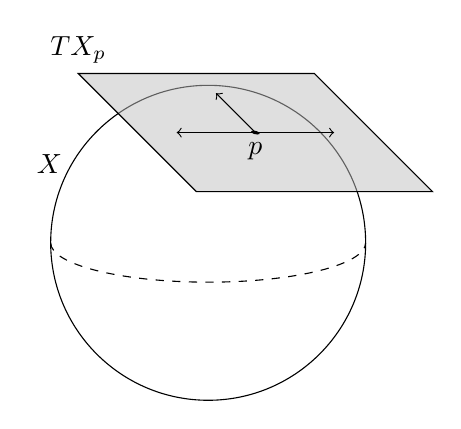
\begin{tikzpicture}
	\draw (0,0) circle (2);
	\draw[dashed] (-2,0) arc[start angle=180, end angle=360, x radius=2, y radius=0.5];

	\coordinate (p) at (0.6,1.4);
	\begin{scope}[y={(-0.5,0.5)}]
		\filldraw[fill=gray!50, fill opacity=0.5] ($ (p) + (-1.5,-1.5) $) -- ($ (p)
		+ (1.5,-1.5) $) -- ($ (p) + (1.5,1.5) $) -- ($ (p) + (-1.5,1.5) $) --
		cycle;
		\draw[->] (p) -- ($ (p) + (-1,0) $);
		\draw[->] (p) -- ($ (p) + (1,0) $);
		\draw[->] (p) -- ($ (p) + (0,1) $);
		\fill (p) circle (0.05) node[below]{$ p $};
		\node[above] at ($ (p) + (-1.5,1.5) $){$ TX_{p} $};
	\end{scope}

	\node[left] at (150:2) {$ X $};

\end{tikzpicture}
\end{document}
